% Created 2022-05-04 Wed 23:46
% Intended LaTeX compiler: pdflatex
\documentclass{IEEEtran}
\usepackage[utf8]{inputenc}
\usepackage[T1]{fontenc}
\usepackage{graphicx}
\usepackage{longtable}
\usepackage{wrapfig}
\usepackage{rotating}
\usepackage[normalem]{ulem}
\usepackage{amsmath}
\usepackage{amssymb}
\usepackage{capt-of}
\usepackage{hyperref}
\usepackage[backend=biber, style=numeric]{biblatex}

\addbibresource{/home/awannaphasch2016/org/papers/org-mode-bibtex.bib}
\author{Anak Wannaphaschaiyong}
\date{\textit{<2022-05-04 Wed>}}
\title{Tokenomics (Cryptoeconomics) and Token Engineering}
\begin{document}

\maketitle

\section{Abstract}
\label{sec:org8ff2ff4}
Blockchain domain evolves very quickly, however, core infrastructure of blockchain has started to mature. For this reason, mental framework to think about blockchain has consolidated. This paper is an introduction to recently emerge subjects: tokenomics and token engineering. The goal of the paper is to provide mental framework to think about tokenomy and to systematically approach evaluation and implement ion of tokenomy via token engineering methodology. The paper discusses significant of blockchain technology that enable tokenomy to materialize and introduce token engineering as a new engineering paradigm and how to approach token design problem. The paper also discusses design components of tokenomics mechanism that is subject to engineering challenge. Lastly, the paper provide framework to evaluate value of tokens.
\section{Introduction}
\label{sec:orgd044103}
Economy is defined as a large set of inter-connected production and consumption activities that drive allocation of scare resources \cite{sowell2014basic}. Economic is a study of economy. Similarly, tokenomic is a study of tokenomy. Tokenomy is defined as tokenized economy. Instead of using money as a medium of exchange that drive participants incentives, tokenized economy uses token.

Any medium of exchange is a form of share believe. Money is a share believe. One can think of money as global shared believe whose value is determined by underlying economy. In tokenomics, token are a share believe within community. One can think of token as local shared believe whose value is determiend by underlying tokenized economy (aka tokenomy). This definition allows one to substitute tokenomics mechanism that composed a tokenomy.

Section \hyperref[sec:org90cbe65]{Evolution of Asset Transaction} explains significant of blockchain technology through the lens of assets transaction evolution. Next, section \hyperref[sec:org77c274b]{Token Engineering (TE)} introduces new paradigm of engineering, called token engineering and explains the needs to adopt engineering practices. Core mechanisms that drive tokenomy are described in \hyperref[sec:org4f1198a]{Tokenomics Mechanism}. Previous section is viewed through the lens of token engineer. In \hyperref[sec:org3c77116]{Evaluate Value of Token} section, we explains how to value token from participants point of view.

\section{Evolution of Asset Transaction}
\label{sec:org90cbe65}
Up until recently, the world has experienced three phases of assets transaction. Blockchain technology enables the next phase. In order, the four phases are transaction of physical assets, transaction of electron, transaction of information, and transaction of digital assets.

Each phase increase efficiency of energy required to complete a transaction which depends on three factors: object, process, and rules. Focusing on economic perspective, one can think of an objects as entities with economic value and process as a automatic process of manipulating objects. Example of processes are movement, composability, and duplication etc. Lastly, rules are constraints imposed upon computation of processes and objects \cite{tai2020nfting}. Using analogy of physic, rules are physic law such as gravity. friction put constraint on movement (process) of objects. Lastly, rules are given. No one can change the rules. However, given a set of rules, object and process can be manipulated.

Equation of object and process are provied as followed

\begin{equation}
\label{asset_transaction_equation}
object = process_1(O, P)
\end{equation}

From equation \ref{asset_transaction_equation}, \(object\) is an output of a process.  \(process\) function take \(O\) and \(P\) as input where \(O\) is a set of \(m\) objects and \(P\) is a set of \(m\) processes and \(n, m \in \mathbb{Z}\).

It is important to understand briefly differences between property, asset, and security. Property is an object that can be owned. Properties of a property is open, permissionless, unsensorable, divisibility, durability, recognizability, scarcity, and portability, see For more information about property \cite{saylor2021bitcoin,breedlove2021philosophy}. Assets is a property that hold economic value. To clarify confusion, security a financial instrument. It is a type of financial asset. Government of a country determines asset that can be categorized as security or non-security.

Each phase of assets transaction evolution create new types of object and new type of process. Wealth of an economy are expanded as new \(object\) and \(process\) are creation. During the first evolution phase, assets are physical assets such as tree and rock. Discovers and inventions of fire, weapon, road, car allows new creation of processes like toasting a bread, chopping tree, and riding a car. In the second phase, ``transaction of electron'' create new objects like electricity, light bulb, and xray and new processes is enable by creation of protocol and communication medium to transfer electricity. With the invention of computer, ``transaction of information'' phase begins. It allows movement of bits and bytes which represent information. This further increases efficiency of communication and exchange of information. However, information alone is not enough to compose and exchange digital assets. The missing puzzle is technology to enable creation of digital property where digital assets can be built on. The technology that allows for the digital assets to be exchanged is blockchain technology. New form of objects includes NFT and crypto. One may argue that digital assets already exists during ``transaction of information'' phase. That's correct. To be clear, blockchain technology doesn't create digital assets. Blockchain technology expands creation of new digital asset and enable digital assets to be transacted.

Crypto currency and token are considered as digital assets. Crypto and money are a form of currency. Crypto is a digital asset whose goal is to substitute money. Token complements both cryptocurrency and money. Recall definition of economy previously defined, economy is an incentive alignment mechanism to allocate scarce assets. On the other hand, tokenomy is tokenized economy. Currency can be thought of as a subset of token, hence economic is a study of homogeneous token economy while tokenomic is a study of heterogeneous token economy such that each tokenize economy has different incentive alignment mechanism.

\section{Token Engineering (TE)}
\label{sec:org77c274b}
\begin{figure}[htbp]
\centering
\includegraphics[width=.9\linewidth]{/home/awannaphasch2016/org/notes/blockchains/images/screenshot_20220504_020205.png}
\caption{\label{tokenomics_sytem}Cryptoeconomic systems are complex socio-economic system.}
\end{figure}

Tokenomics is defined as self-funding mechanism for projects within the token economy. Voshmgir et al. \cite{hellerstein2005anatomy} frame tokenomics as a subfield of economics system, see \ref{tokenomics_sytem}. Voshmgir et al. \cite{voshmgir2020foundations} mentioned that tokenomics' design was subjective and lack rigorous approach and purposed to adopt approaches from existing interdisciplinary field. According to \cite{kreitenweis2021token}, token engineering (TE) disciplinary is the most recent engineering discipline after software engineering. TE was mentioned for the first time in 2018. The goal of TE is to bring engineering practice into tokenomics's design by providing methodology to go from ideation to design, modeling, simulation, testing, deployment, and maintentance. Figure \ref{interdisciplinary_in_tokenomics} shows venn diagram of disciplines that TE can benefit from. Framing TE as a new engineering discipline allows researchers to adapt large body of existing literature and avoid reinvent the wheel.


\begin{figure}[htbp]
\centering
\includegraphics[width=.9\linewidth]{/home/awannaphasch2016/org/notes/blockchains/images/screenshot_20220504_022613.png}
\caption{\label{interdisciplinary_in_tokenomics}Interdisciplinary in token engineering. The image is taken from \cite{voshmgir2020foundations}.}
\end{figure}

\subsection{Incentive Layers}
\label{sec:orgf659cdf}
Given functional layer is implemented, incentive layer make sure that members are incentivized to perform unharmful action such that constraints in functional layer is obeyed.

Steps to design and economic game is the following \footnote{\href{https://www.youtube.com/watch?v=gCFlGLbI\_kE\&ab\_channel=TechCrunch}{Sam Williams: Mechanism Design 101}}
\begin{enumerate}
\item Choose a goal
\item Choose a reward mechanism
\item Choose a reward function to match it.
\end{enumerate}

\subsubsection{Game theory}
\label{sec:org8cf8696}
Game theory are useful in DAO design because it involve interaction of many participants. Design of game theory is categorized into player design and mechanism design. Player design optimize player decisions to maximize their utility gain. Player design goals is to establish equilibrium (e.g. Perfect equilibrium and Nash equilibrium). Effort in player design is put toward finding Nash equilibrium. Nash equilibrium is established when there is no incentive to deviate from the initial strategy to reach optimal outcomes for all players. On the other hand, mechanism design theory studies the mechanisms by which a particular outcomes and results can be achieved. Mechanism design doesn't need to account for equilibrium. Intuitively, the desired outcome can be reached if players doesn't make bad action. In this case, there is no need for players to find the best action.

Game theory should be designed for all weather of the markets. Participants have different incentive to join or abandon the project as market rises and fall.

One common strategy of tokenomic game theory is ``lockups.'' lockups is a mechanism employed by staking. When staking on tokens, the protocol creates and incentive for locking your tokens in a contracts which will return some form of reward in return. This lockups is a form of ``conviction voting'' \cite{honkanen2021organizational} that is used outside of governance mechanism. Conviction voting is one of many voting mechanism of DOA governance \cite{honkanen2021organizational}. This form of voting goals is to weighted value of vote by time the vote has been submitted for

Game-theoretic approach simplifying assumption imposed by designer knowledge. For this reason, it is difficult to incorporate non-rationality. Furthermore, this disable tokenomics mechanism to evolve to adapt to unknown and unknown unknown. Even when designers have an opportunity to adapt the system, game-theoretic approach requires high computation over-head causing necessary but inevitable delay which allows the problem to amplify its damage or emerge into new and bigger problem.

Incentivai approach the problem by provides parameters to AI models and delegate responsibility of optimization to AI models \cite{grudzien2019incentive}. This approach doesn't simplify dynamic nature of the problems. However, assumptions still exists. The assumptions lie in hyper-parameters of AI models and capability of AI models to find optimal solution. Therefore, instead of training AI end-to-end, AI models can be used as tools to explore optimal strategies outside of the game-theoretic solution. In summary, AI models can substitute mathematical models as optimization components within TE framework.

[explain TE frameworks]

\subsubsection{Mechanism Design}
\label{sec:org20c051c}
Mechanism design is a subfield of game theory. Mechanism design in decentralize system is harder to terminate/update/recovery than in centralized system.
Example of this problem is bitcoin block size that is programmed to have 1M limit as a results people demand to bit for their transaction to be included in the block and drive up rewards per block which is a great news for miner. For this reason, there is no incentive for miner to agree on increase the block size.
\subsubsection{Problem with game theory an mechanism design}
\label{sec:org71d23b1}
Game theory assumes that game is static, but tokenomics games are not static. To deal with dynamic system, focus should be on control system. This bring back to optimization and to evolutionary algorithm. The goal that should be focus on is how to control evolution of the game and try to understand how it evolves and what it can and cannot evolve. To understand evolution of emergent system, one must find property of the system then add property as a requirement to constraint of the desired system. The iteration continue. This process continuously and systematically narrow down incentives space towards desired behavior.
\subsubsection{Case Study: Incentive alignment in Ethereum}
\label{sec:org9ff249f}
This section discuss how tokenomic intertwined with economic. To make concrete example. we will use Ether and proof of work (at the time of writing Ethereum still uses proof of work) as an example.
\begin{enumerate}
\item Gas and Denominations of coins
\label{sec:orgfe24fe0}
\begin{figure}[htbp]
\centering
\includegraphics[width=.9\linewidth]{/home/awannaphasch2016/org/notes/blockchains/images/screenshot_20220315_124959.png}
\caption{\label{fig:img}Denominations of Ethers. Image is borrowed from Etherem yellow paper.}
\end{figure}

In this section, we will focus on denominations of Ethers. The goal is to provide more concrete example into denomination of a coin. According to Etherem yellow paper (aka technical white paper)  \cite{wood2014ethereum}, list of all denominators of Ether is shown in Fig. \ref{img}.

These denominators are units of gas cost in transaction. When discussion about cost of gas, using GWei is more convenience, hence, a more widely use as a unit of gas price. Transaction cost is calculated as (amount of gas \(\times\) cost per unit of gas.)

Still, It is important to talk about mechanism in which Wei is value.
Wei value is calculated based on demands of transaction and supply of gas, more on economy of blockchain this later.

The idea behind gas is to make user pays for computational resources required to complete a transaction on a blockchain. An incentive alignment mechanism is designed to influence demands of a user to run the transaction and pay for computation cost of a smart contract \cite{el2021decentralized}.
\item Optimizing number of gas supply of blockchain at a given point in time.
\label{sec:org0f8787a}
Since number of gas available is equivalent of supply, and production of supplies depend on block size (gas limit per block) and times it take to validate the block (difficulty of the block puzzle). To maximize number of gas supply, we can adjust difficulties of block puzzle such that equation \ref{gas_supply_eq} is maximize \cite{wood2014ethereum}.


\begin{equation}
\label{gas_supply_eq}
\text{gas supply }= \text{number of block } \times \text{ size of block }
\end{equation}

The level of difficulties also has to take into account mining power per time unit. Therefore, at a given point in time, we are given mining power per time unit and we have to solve for difficulties that maximize number of gas supply. See the problem statement below for clarification.

\begin{verbatim}
Problem statement
-----------------

Given (mining power per time unit),
we must solve for optimal level of
(puzzle difficulties) such that
(size of block) and (number of blocks)
will results in maximum number of gas
supplies

Base on the following requirement.
1. solving more difficult puzzle results
   in less number of block per time
   interval.
2. equation 2
\end{verbatim}

Difficulty level has the following formula \cite{wood2014ethereum}.

\begin{equation}
Difficulty\_level = HashRate / Constant
\end{equation}

\(HashRate\) is the ``mining power per time unit'' we mentioned above.

It is important to note that \(HashRate\) cannot be calculated in real time instead it newly generate per cycle which is about 14 days. Hence, calculation of \(HashRate\) lags behind actual supply and demand in the market.

\item What is the incentive to mine?
\label{sec:org19ddf61}
As we mentioned above that supply of gas controlled by \(HashRate\), but what exactly is the underlying incentives for mining? the answer is tokens as minning's reward. For every time block puzzle is solved, fixed number of ``reward'' is given to miner in the form of tokens. To sum up, solving a block puzzle generate reward to the miner as in the form of tokens and these same tokens are added to the economy as supply of blocks that contains gas. Furthermore, the token itself is an asset which contain value and are tradable whose value is controlled by ``coins markets''.

value of coin markets is determined by economy of computation and computation market is determined by economy of coins. Computation market is the market that involves miner, smart contract, and gas. Miners supplies gas by solving puzzle (aka mining). Smart contract can be thought of as demand in the market because number gas must be paid as a cost to compute these smart contracts. Lastly, gas is the entity whose value is calculated as \$ \text{price of Gwei } \(\times\) \text{ number of Gwei}\$ and is used to value cost of transaction.

``Coin market'' is the market that involves coins owner (which may or may not be miners themselves, coins buyer, and coins. Coin owners are those who possess coins. Coins buyers are those who wants to be the future owner of the coins. Lastly, coins is an entity that hold monetary values and can use as transfer of wealth.

The only factor that tight the market together is ``incentive of the miner.'' miners mine coins because coin can be traded in the ``coin market'' with ``real money''. And it just happens that the mined coins are, in facts, consist of blocks which provide supply to the ``computation market.''
\end{enumerate}

\section{Tokenomics Mechanism}
\label{sec:org4f1198a}
Tokenomics mechanism is incentive alignment mechanism. There are two mains tokenomics mechanism: fair token distribution and token bonding curve. The idea of tokenomics mechanism is to use financial incentive to compensate for the lack of utility. Example of utilities could be bootstraping phase to bring new users and contributor on board.

\subsection{Fair Token Distribution.}
\label{sec:org2333947}
Main goal of token distribution should be to maximize token distribution to potential users and contributors. Unfairness in token distribution stage, which is the first stage of tokenomics, have compounded effects overtimes \cite{daly2019why}.

Token distribution mechanism are mining, ICOs, AirDrops Markle mine, and lock drop \cite{daly2019why} .
Mining goal is fair and wide distribution with easy access. Problem with mining is that token can be pre-mined and imbalance of information distribution on how and when to mine and associated risk such as solvers take partial reward, miner extractable value (MEV), from miners. AirDrop solve information imbalance by simply giving away free token. However, this attracts less enthusiastic people which increase risk of idle and decrease token circulation. ICO (token sale) solve information imbalance and token idleness by allowing investors to buy token during token sale. However, ICO is a form of fund raising. Existing problem of fund raising is wealth imbalance, where richer individuals can buy more token, which leads to concentration of power defeating purposing of decentralization. Lock drop allows user to stake target token with other tokens. Recall that staking earns token holder cash flow as passive income without selling token. It is equivalent of a high-yield saving account.

\subsection{Token Bonding Curve}
\label{sec:orgd16dae1}
In simple word, bonding curve is a function that take token as input and output different token. Bonding curve enable token model that allow community to create wealth together by solving coordination problem. This is done by creating reward and cost for information sharing. In another word, token bonding curve is a function of token supply, cost of communication, and protocol automation cost.

\begin{center}
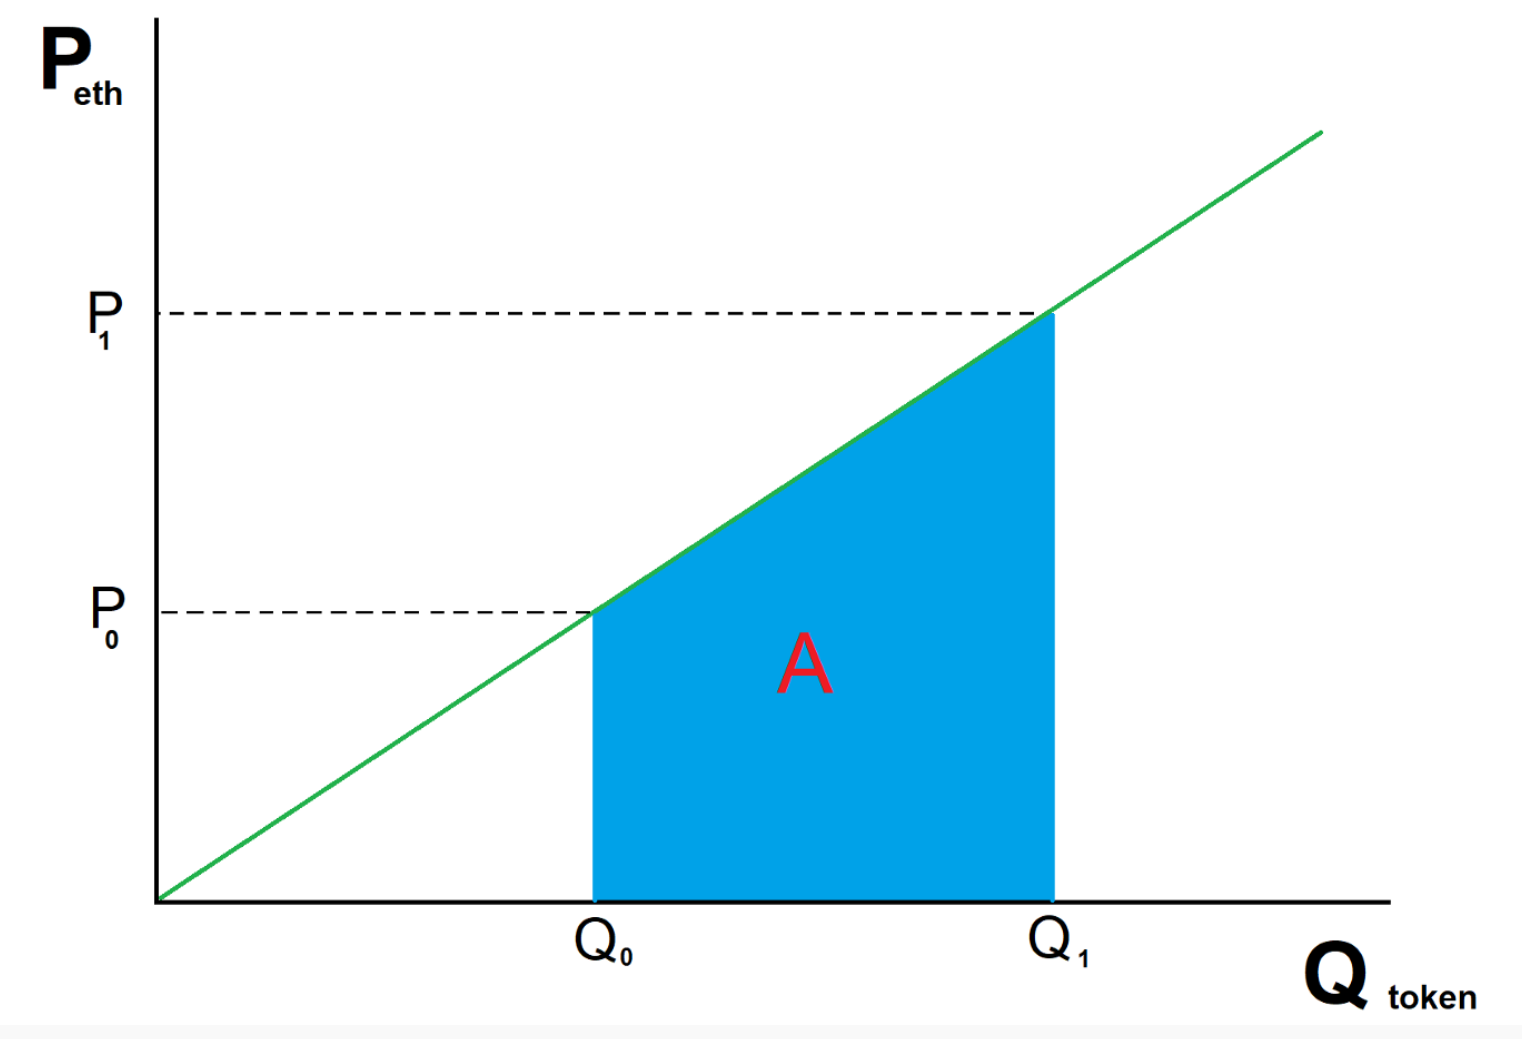
\includegraphics[width=.9\linewidth]{./images/screenshot_20220504_233447.png}
\end{center}

\section{Evaluate Value of Token}
\label{sec:org3c77116}
Value of token is reflected from equivalent fiat currency value owned. According to price discovery mechanism \cite{walsh2017monetary}, price of a supply can be calculated from two demand functions and supply functions.
\subsection{Demand Mechanism}
\label{sec:org28ee683}
One can get evaluate utility of a token. There are four types of utility: Spending vs Holding, Cash flows, Governance, and Collateral \cite{eliason2022tokenomics}.

Some tokens are designed to be either spent (spending token) or hold (holding token).
Utility of holding token depends on supply and demands of the token itself. This is equivalent to money. In the other word, token as an medium of exchange. On the other hand,

Designing purpose for spending token is such that the token itself has no holding utility. In the other word, tokens should be bought to spent. The faster one spends the token, the less opportunity cost the token creates --- there is no cash flow or other utilities while holding token. Spending token must be spent to realized utility gain. This is rather a common usecase in real life. Imagine a concert ticket. The ticket utility is to get an individual into a concern. That's all its utility. There are a period where the prices of ticket fluctuate due to demand-supply right before the concert started. After the concert is finished, utility and demands reaches zero. Example of spending token is \$LINK token which is used to buy Chainlink's services, see figure \ref{$LINK} for \$LINK token historical prices. When analyses price level of a spending token, one should think from token designer's point of view. In the case of \$LINK, Chainlink doesn't want its services to be expensive, hence Chainlink may implement mechanism to keep the price low.

\begin{figure}[htbp]
\centering
\includegraphics[width=.9\linewidth]{/home/awannaphasch2016/org/notes/blockchains/images/screenshot_20220423_114515.png}
\caption{\label{$LINK token historical prices.}An example of holding token prices. \$LINK token is used to buy Chainlink's services.}
\end{figure}

\subsubsection{Cash flows from holding token}
\label{sec:org3e19d67}
If you decide to hold a token, what is the utility that holding token should bring? The obvious reason is to increase in values of total token holds in the future. Total value of token in blockchain project increase is via incentives engineering either by
\begin{enumerate}
\item Discouraging people from selling your token
\item Encouraging people to buy the token.
\end{enumerate}

To increase value of total tokens,

\subsection{Supply Mechanism}
\label{sec:org1c960a6}
This mechanism concerns inflation/deflation components of token which is a function of the following factors: number of existed token, token in circulation, token distribution, unlock schedule of remaining token. Token mechanism that can effect token values are burns and split. There are token mechanisms that amplify return of investment (ROI) by utilizing staking, among other.

Evaluating token supply requires asking the following question.
\begin{enumerate}
\item Where is the supply right now?
\item Where will it be in the future?
\item When will it be there?
\item How will it get there?
\end{enumerate}

\subsubsection{Initial Token distribution}
\label{sec:orgef69078}
Token distribution describes the proportions in which ownership is distributed among different groups of users. Figure \ref{intial_token_allocation_for_public_blockchain} show intial token allocation for public blockchain. The figure is borrowed from Messari website.

\begin{figure}[htbp]
\centering
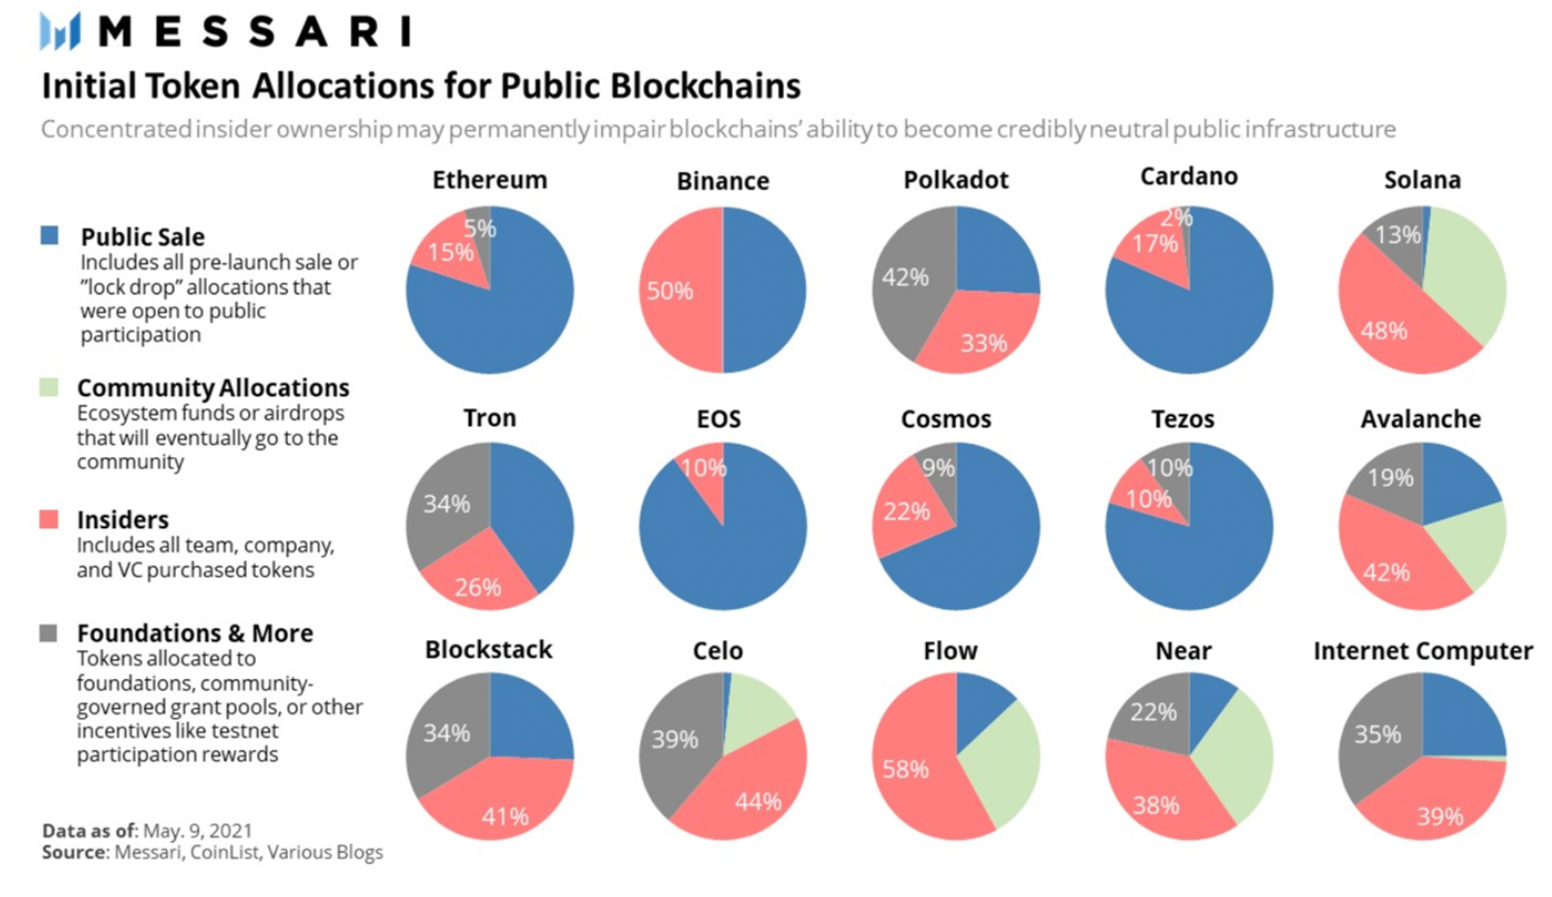
\includegraphics[width=.9\linewidth]{./images/screenshot_20220504_231549.png}
\caption{\label{intial_token_allocation_for_public_blockchain}intial token allocation for public blockchain}
\end{figure}

\subsubsection{Supply Metrics}
\label{sec:org43578dd}
The market cap and the fully diluted valuation (FDV) are the two common metrics. The market cap measure total value of all tokens at the current time point while FDV measure total value of all token of all possible supply that can be produced.

The market cap is the circulating supply of tokens multiplied by the token price. The FDV is the current price multiplied by the max supply, if all tokens were in circulation.

A way to think of this is if the market cap is 10\% of the FDV and the tokens are all released in the next year. Project will have to grow 10x to maintain its current price. So the question one should ask before invest in the project long term is ``Will price of cost increase by 10x when all supply is released?''

\subsubsection{Supply Circulation}
\label{sec:orga0e6406}
Knowing number of tokens released at a given point in time is not enough. Price discovery, according to monetarist theory, is formulate as \(PQ=MV\) where \(P\) is price per unit of supply, \(Q\) is quantity of supply, \(M\) is money and \(V\) is value \cite{walsh2017monetary}. Velocity of the token circulation is also important. Velocity depends on circulating supply. circulating supply is a supply of actively traded token. ``Inactivity'' of token calculation differs between information platforms supplying the API as seen in figure \ref{circulating_supply_of_$RAIDER} and figure \ref{circulating_supply_of_$CRV}.

\begin{figure}[htbp]
\centering
\includegraphics[width=.9\linewidth]{/home/awannaphasch2016/org/notes/blockchains/images/screenshot_20220422_224334.png}
\caption{\label{circulating_supply_of_$RAIDER}circulating supply of \$RAIDER}
\end{figure}

\begin{figure}[htbp]
\centering
\includegraphics[width=.9\linewidth]{/home/awannaphasch2016/org/notes/blockchains/images/screenshot_20220422_224500.png}
\caption{\label{circulating_supply_of_$CRV}circulating supply of \$CRV}
\end{figure}

\subsubsection{Supply Expansions and Contractions Mechanism}
\label{sec:org8d1144d}
Emission rates is a mechanism of injecting new tokens into the circulation. The impact of emission rates depends heavily on the initial token distribution plan. This is because often time token emission are release based on percentage of total tokens. Emission schedules can either be static or dynamic. Static emission schedules of JonesDAO is shown in figure \ref{JonesDAO's_emission_rates_overtime}. According to \ref{JonesDAO's_emission_rates_overtime}, during the displayed preriod, the inflation rate will be more than doubled. And the new tokens entering the market will exclusively be going to people who got in at a heavily discounted price. Furthermore, dynamic emission schedule of Convex (\$CVX) is shown in figure \ref{Convex_emission_rate_overtime}. \$CVX emission rate is a function of CRV rewards farmed by Convex \cite{covex2021tokenomics}, hence the name performance-based emission. Covex is a liquidator platform and farming is a Defi's terminology meaning staking on assets to be put in the liquidity pools.

\begin{figure}[htbp]
\centering
\includegraphics[width=.9\linewidth]{/home/awannaphasch2016/org/notes/blockchains/images/screenshot_20220422_225225.png}
\caption{\label{JonesDAO's_emission_rates_overtime}JonesDAO's emission overtime}
\end{figure}
\begin{center}
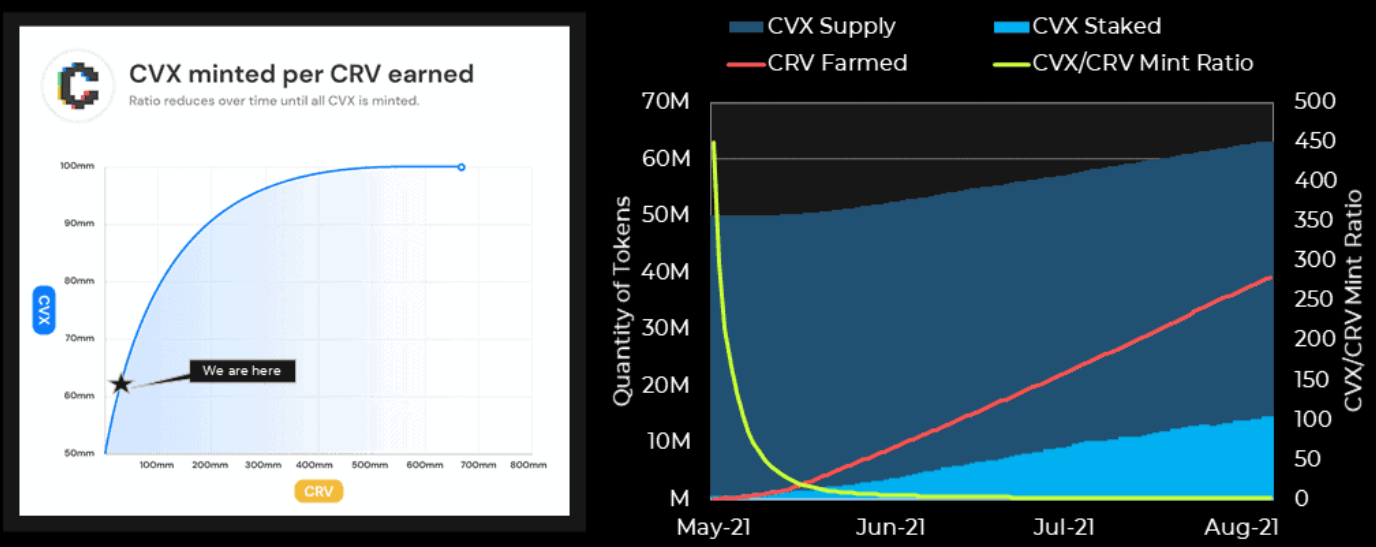
\includegraphics[width=.9\linewidth]{./images/screenshot_20220504_223846.png}
\label{Convex_emission_rate_overtime}
\end{center}

\section{Conclusion}
\label{sec:orgabc1d4e}
The paper provide mental framework to think about significant of blockchain technology by explaining evolution of asset transaction. Then, the paper explains token engineering methodology and justifies the need to adopt engineering practices. Furthermore, multiple tokenomics mechanism is explained. Lastly, the paper discuss framework to analyze value of token.

\printbibliography
\end{document}
